\chapter{Klausurtraining}

\setcounter{section}{15}
\setcounter{subsection}{0}
\setcounter{subsubsection}{1}
\setcounter{secnumdepth}{4}
\subsection{Klausurtipps}
\href{https://youtu.be/uMfjDH8dFl4}{Video 01}\\
Klausurvorbereitungzeit  (Zeitaufwand ca. 7-10 Tage, a 5-8 Stunden):\\

\begin{tabular}[t]{ll}% l=linksbündig r=rechtsbündig
	\textbullet & Alle wichtigen Sätze in einer Zusammenfassung aufschreiben.  \\
	&\\
	\textbullet&Alle Aufgaben aller Aufgabenblätter alleine durchgehen und bearbeiten und danach mit\\
	& Musterlösung vergleichen. \\
	& Liste von problematischen Aufgaben erstellen.\\
	&\\
	\textbullet&Bearbeite alle relevanten Aufgaben aus der Vorlesung.\\
	&Liste von problematischen Aufgaben erstellen.\\
	&\\
	\textbullet&Bearbeite Altklausuren\\
	&\\
	\textbullet&Listen durchgehen\\
	&\\
	\textbullet&Simuliere Klausursituationen\\
	&\\
\end{tabular}\\
\\
In der Klausur:\\

\begin{tabular}[t]{ll}% l=linksbündig r=rechtsbündig
	\textbullet & Überfliege Klausur und schätze Schwierigkeitsgrad der Aufgaben ein.  \\
	&\\
	\textbullet&Bearbeite Klausur von \glqq leicht nach schwer\grqq durch.\\
	&\\
	\textbullet&Lese Aufgabenstellung gründlich und überlege eine Strategie\\
	&zur Bearbeitung und fange dann an!\\
	&\\
	\textbullet&Ruhig bleiben: Bei Fehlern mit falschen Ergebnissen weiter rechnen.\\
	&\\
	\textbullet&Schreibe keinen \glqq Quatsch\grqq: Z.B. keine allgemeine Formel.\\
	&\\
\end{tabular}\\
\\
Nach der Klausur: Gehe in die Einsicht!
\newpage
\noindent
\subsection{Aufgabe 1 - Komplexe Zahlenmenge}
\href{https://youtu.be/mBNzaQIcrM8}{Video 02}\\
Skizziere folgende Menge in der Gauß'schen Zahlenebene:\\
\begin{align*}
\{ z\in\mathbb{C} \;|\; z^4 =8\sqrt{2} (1+\mathrm{i})  \}\cap\{ z\in \mathbb{C}\;|\;  |z| \leq 2 \}
\end{align*}
\underline {Bestimmung der Menge: $  \mathbb{A} $}\\
\begin{align*}
\mathbb{A}:=\{ z\in\mathbb{C} \;|\; z^4 =8\sqrt{2} (1+\mathrm{i})  \}\
\end{align*}
\begin{quote}
	\textbullet\;\;Lösen von $z^4 =8\sqrt{2} (1+\mathrm{i})  $\\
	\begin{quote}
		Es gilt:\\\\
		\begin{align*}
		z^n&=|a|\cdot\mathrm{e}^{\mathrm{i}\alpha}\\
		z_k&=\sqrt[n]{|a|}\cdot\mathrm{e}^{\mathrm{i}\frac{\alpha+2k\pi}{n}}\;\;\text{für }\;\;k=0,1,2,\ldots,n-1
		\end{align*}
		\underline{Darstellung der komplexen Zahl $ a=8\sqrt{2}(1+\mathrm{i}) $ in Polarkoordinaten.}\vspace*{4mm}	\\
		Bestimmung des Betrage von $ |a| $.\\
		\begin{align*}
		|a|=|8\sqrt{2}(1+\mathrm{i})|=8\sqrt{2}|(1+\mathrm{i})|=8\sqrt{2}\cdot\sqrt{|1^2|+|\mathrm{i}^2|}=8\sqrt{2}\sqrt{1^2+1^2}=8\sqrt{2}\sqrt{2}=8\cdot 2=16
		\end{align*}
		
		Bestimmung des Winkels $ \alpha $:\\
		\begin{center}
			
			
			\begin{tikzpicture}[xscale=1, yscale=1]
			
			% Gitternetzlinien
			%\draw[xstep=1cm, ystep=1cm, very thin, color=lightgray] (-4,4) grid (4,-2);
			% x-Achse
			\draw[->] (-4,0) -- (4,0) node[below,xshift=-1em] {Re}; 
			
			% y-Achse 
			\draw[->] (0,-2) -- (0,4) node[left,yshift=-1em] {Im};%node[above left]
			\draw[color=blue] (1.5,0.8)  node[below] {$ \alpha =\frac{\pi}{4} $}; 
			\draw[color=green, ->] (0.6,0) arc (0:180:0.6);
			\draw[color=blue, ->] (1,0) arc (0:45:1);
			\draw[color=green] (-1.2,0.8)  node[below] {$ \beta =\pi $}; 
			\draw[thick,->,color=blue] plot[samples=200, domain=0:2] 
			(\x,{\x}) node[below, xshift=1em]{$\overrightarrow{a} $};
			\end{tikzpicture}
		\end{center}
		Nach Skizze folgt: $ \alpha=\frac{\pi}{4} $
		
	\end{quote}
	Nun kann man die Gleichung lösen mit:\\
	\begin{align*}
	z_k&=\sqrt[n]{|a|}\cdot\mathrm{e}^{\mathrm{i}\frac{\alpha+2k\pi}{n}}\;\;\text{für }\;\;k=0,1,2,\ldots,n-1\\
	z^k&=\sqrt[4]{16}\cdot\mathrm{e}^{\mathrm{i}\cdot \frac{\frac{\pi}{4}+2k\pi}{4}}\\
	z^0&=2\cdot \mathrm{e}^{\mathrm{i}\cdot\frac{\pi}{16}}\\
	z^1&=2\cdot \mathrm{e}^{\mathrm{i}\cdot\frac{\pi}{16}+\frac{\pi}{2}}\\
	z^2&=2\cdot \mathrm{e}^{\mathrm{i}\cdot\frac{\pi}{16}+\pi}\\
	z^3&=2\cdot \mathrm{e}^{\mathrm{i}\cdot\frac{\pi}{16}+\frac{3\pi}{2}}\\
	\end{align*}
	Daraus folgt:\\
	\begin{align*}
	\mathbb{A}=\{z_0,z_1,z_2,z_3\}
	\end{align*}
	Skizze von der Menge $ \mathbb{A} $:\\
	\begin{center}
		
		
		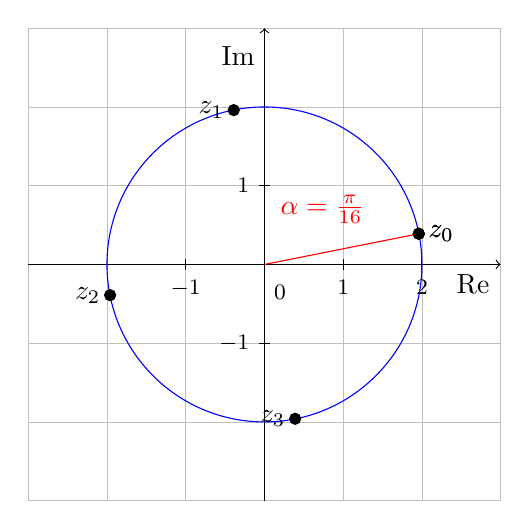
\begin{tikzpicture}[xscale=1, yscale=1]
		
		% Gitternetzlinien
		\draw[xstep=1cm, ystep=1cm, very thin, color=lightgray] (-3,3) grid (3,-3);
		% x-Achse
		\draw[->] (-3,0) -- (3,0) node[below,xshift=-1em] {Re}; 
		%Zahlen auf x-Achse
		\foreach \x in {-1,...,-1}
		\draw[shift={(\x,0)},color=black] (0pt,2pt) -- (0pt,-2pt) node[below] {\footnotesize $\x$};
		\foreach \x in {1,...,2}
		\draw[shift={(\x,0)},color=black] (0pt,2pt) -- (0pt,-2pt) node[below] {\footnotesize $\x$};
		% y-Achse 
		\draw[->] (0,-3) -- (0,3) node[left,yshift=-1em] {Im};%node[above left]
		%Zahlen auf y-Achse
		\foreach \y in {-1,...,-1}
		\draw[shift={(0,\y)},color=black] (2pt,0pt) -- (-2pt,0pt) node[left] {\footnotesize $\y$};
		\foreach \y in {1,...,1}
		\draw[shift={(0,\y)},color=black] (2pt,0pt) -- (-2pt,0pt) node[left] {\footnotesize $\y$};
		%Ursprung
		\draw[color=blue] (2,0) arc (0:360:2);
		\draw[color=black] (0pt,-10pt) node[right] {\footnotesize $0$};
		\draw[color=red] (0,0)--(1.96,0.39);
		\filldraw[black] (1.96,0.39) circle (2pt) node[anchor=west] {$ z_0 $};\filldraw[black] (1.96,0.39) circle (2pt) node[anchor=west] {$ z_0 $};
		\filldraw[black] (-1.96,-0.39) circle (2pt) node[anchor=east] {$ z_2 $};
		\filldraw[black] (-0.39,1.96) circle (2pt) node[anchor=east] {$ z_1 $};
		\filldraw[black] (0.39,-1.96) circle (2pt) node[anchor=east] {$ z_3 $};
		\draw[red] (1.39,0.7)  node[anchor=east] {$\alpha=\frac{\pi}{16} $};
		\end{tikzpicture}
	\end{center}
	Die Menge: $ \mathbb{A}=\{z_0,z_1,z_2,z_3\} $ ist auf dem Kreis mit Radius: $ r=2 $.\\
\end{quote}
\underline{Bestimmung der Menge: $ \mathbb{B} $}\\
\begin{quote}
	\begin{align*}
	\mathbb{B}=\{ z\in \mathbb{C}\;|\;  |z| \leq 2 \}
	\end{align*}
	Es gilt:\\
	\begin{align*}
	\mathbb{B}=\{x+\mathrm{i}y\in \mathbb{C}\;|\;\sqrt{x^2+y^2}\leq 2\}
	\end{align*}
	$ \sqrt{x^2+y^2} $ ist eine Kreisscheibe mit Radius: $ r=2 $ um $ (0,0) $.\\
	\begin{center}
		
		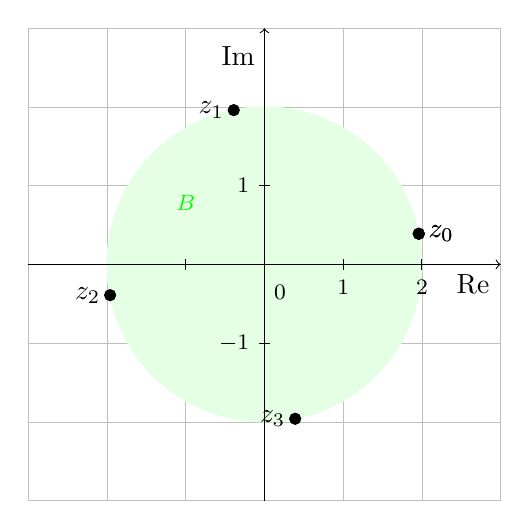
\begin{tikzpicture}[xscale=1, yscale=1]
		
		% Gitternetzlinien
		\draw[xstep=1cm, ystep=1cm, very thin, color=lightgray] (-3,3) grid (3,-3);
		\filldraw[color=green!10] (2,0) arc (0:360:2);
		\draw[color=green](-1,1)node[below]{\footnotesize $\mathbb{B}$};
		% x-Achse
		\draw[->] (-3,0) -- (3,0) node[below,xshift=-1em] {Re}; 
		%Zahlen auf x-Achse
		\foreach \x in {-1,...,-1}
		\draw[shift={(\x,0)},color=black] (0pt,2pt) -- (0pt,-2pt) ;
		\foreach \x in {1,...,2}
		\draw[shift={(\x,0)},color=black] (0pt,2pt) -- (0pt,-2pt) node[below] {\footnotesize $\x$};
		% y-Achse 
		\draw[->] (0,-3) -- (0,3) node[left,yshift=-1em] {Im};%node[above left]
		%Zahlen auf y-Achse
		\foreach \y in {-1,...,-1}
		\draw[shift={(0,\y)},color=black] (2pt,0pt) -- (-2pt,0pt) node[left] {\footnotesize $\y$};
		\foreach \y in {1,...,1}
		\draw[shift={(0,\y)},color=black] (2pt,0pt) -- (-2pt,0pt) node[left] {\footnotesize $\y$};
		%Ursprung
		%\filldraw[color=green] (2,0) arc (0:360:2);
		
		\draw[color=black] (0pt,-10pt) node[right] {\footnotesize $0$};
		%\draw[color=red] (0,0)--(1.96,0.39);
		\filldraw[black] (1.96,0.39) circle (2pt) node[anchor=west] {$ z_0 $};\filldraw[black] (1.96,0.39) circle (2pt) node[anchor=west] {$ z_0 $};
		\filldraw[black] (-1.96,-0.39) circle (2pt) node[anchor=east] {$ z_2 $};
		\filldraw[black] (-0.39,1.96) circle (2pt) node[anchor=east] {$ z_1 $};
		\filldraw[black] (0.39,-1.96) circle (2pt) node[anchor=east] {$ z_3 $};
		%\draw[red] (1.39,0.7)  node[anchor=east] {$\alpha=\frac{\pi}{16} $};
		
		\end{tikzpicture}
	\end{center}
\end{quote}
\underline{Bestimmung von $ \mathbb{A}\cap\mathbb{B} $}\\
\begin{quote}
	Es gilt:\\
	\begin{align*}
	\mathbb{A}\subset\mathbb{B}\Rightarrow\mathbb{A}\cap\mathbb{B}=\mathbb{A}
	\end{align*}
\end{quote}
\subsection{Aufgabe 2 - Grenzwert einer Folge}
\href{https://youtu.be/360OQSMzKcc}{Video 03}\\
Bestimme den Grenzwert folgender Folge:\\
\begin{align*}
x_n:=\frac{\pi\cdot n^3+\cos(n^2)}{4\cdot n^3-\sin(\frac{1}{y})}
\end{align*}
Betrachte:\\
\begin{align*}
x_n&=\frac{\pi\cdot n^3+\cos(n^2)}{4\cdot n^3-\sin(\frac{1}{y})}\\
&=\frac{n^3(\pi+\frac{\cos(n^2)}{n^3})}{n^3(4-\frac{\sin(\frac{1}{n+1})}{n^3})}\\
\lim\limits_ {n\to\infty} x_n&=\frac{\pi+\overbrace {\frac{\cos(n^2)}{n^3}}^{\rightarrow 0}}{4-\underbrace{\frac{\sin(\frac{1}{n+1})}{n^3}}_{\rightarrow 0}}=\frac{\pi}{4}
\end{align*}
\newpage
\noindent
\subsection{Aufgabe 3 - Grenzwert einer Folge}
\href{https://youtu.be/ICQcFrINxAQ}{Video 04}\\
Bestimme den Grenzwert folgender Folge:\\
\begin{align*}
x_n:=\sqrt{2n}\big(\sqrt{n+1}-\sqrt{n}\big)
\end{align*}
Betrachte:\\
\begin{align*}
x_n&=\sqrt{2n}\big(\sqrt{n+1}-\sqrt{n}\big)\\
&=\sqrt{2n}\frac{\big(\sqrt{n+1}-\sqrt{n}\big)\big(\sqrt{n+1}+\sqrt{n}\big)}{\big(\sqrt{n+1}+\sqrt{n}\big)}\\
&=\sqrt{2n}\frac{n+1-n}{\big(\sqrt{n+1}+\sqrt{n}\big)}\\
&=\sqrt{2}\sqrt{n}\frac{1}{\big(\sqrt{n+1}+\sqrt{n}\big)}\\
&=\sqrt{2}\frac{\sqrt{n}}{\big(\sqrt{n+1}+\sqrt{n}\big)}\\
&=\sqrt{2}\frac{\sqrt{n}}{\sqrt{n}\bigg(\frac{\sqrt{n+1}}{\sqrt{n}}+1\bigg)}\\
&=\sqrt{2}\frac{\sqrt{n}}{\sqrt{n}\bigg(\sqrt{\frac{n+1}{n}}+1\bigg)}\\
&=\sqrt{2}\frac{\sqrt{n}}{\sqrt{n}\bigg(\sqrt{\frac{n(\frac{1}{n}+1)}{n}}+1\bigg)}\\
&=\sqrt{2}\frac{1}{\bigg(\sqrt{\frac{1}{n}+1)}+1\bigg)}\\
&=\sqrt{2}\frac{1}{2}=\frac{\sqrt{2}}{2}
\end{align*}
\subsection{Aufgabe 4 - Induktion}
\href{https://youtu.be/nJx5VsSVHaQ?t=5}{Video 05}\\
Beweise mit vollständiger Induktion:\\
\begin{align*}
\sum\limits_{k=1}^{n}k(k+1)=\frac{n(n+1)(n+2)}{3}\;\;\text{ für}\;\;n\in\mathbb{N}
\end{align*}
$ \bullet $\;\;(I.A.):\\
\begin{quote}
	Für $ n=0 $ gilt:\\
	\begin{align*}
	\sum\limits_{k=0}^{0}k(k+1)=0=\frac{0(0+1)(0+2)}{3}\checkmark
	\end{align*}
\end{quote}
$ \bullet $\;\;(I.V.):\\
\begin{align*}
\sum\limits_{k=1}^{n}k(k+1)=\frac{n(n+1)(n+2)}{3}\;\;\text{gilt für \underline{ein} }\;\;n\in\mathbb{N}
\end{align*}
$ \bullet $\;\;(I.S.):\\
\begin{quote}
	Z.z.:
	\begin{align*}
	\sum\limits_{k=1}^{n+1}k(k+1)=\frac{(n+1)(n+2)(n+3)}{3}
	\end{align*}
	Es gilt:\\
	\begin{align*}
	\sum\limits_{k=1}^{n+1}k(k+1)=	\sum\limits_{k=1}^{n}k(k+1)+(n+1)(n+2)&\overset{(I.V.)}{=}\frac{n(n+1)(n+2)}{3}+(n+1)(n+2)\\
	&\;\;=\frac{n(n+1)(n+2)+3(n+1)(n+2)}{3}\\\sum\limits_{k=1}^{n+1}k(k+1)&\;\;=\frac{(n+1)(n+2)(n+3)}{3}\boxed{}\\
	\end{align*}
\end{quote}

\subsection{Aufgabe 5 - Differenzierbarkeit}
\href{https://youtu.be/8EBDpt2f5S0}{Video 06}\\
Für welches $ \alpha=\in\mathbb{R} $ ist $ f:\mathbb{R}\mapsto \mathbb{R}$ mit\\

\begin{align*}
f(x) =     \left\{ \begin{array}{rcl}
x\cdot\mathrm{e}^{\sinh(x)} +\alpha(x+1)& \mbox{für} & x\geq0\\
-1&\mbox{für} & x<0
\end{array}\right.
\end{align*}
in $ x_0=0 $ differenzierbar.\\
\\
Der Grenzwert des Differntialquotienten muss links von $ x_0=0 $ und rechts von $ x_0=0 $ gleich sein.\\
Es muss gelten:\\
\begin{align*}
\lim\limits_ {\substack{x\to x_0\\x>0}}\frac{f(x-f(x_0))}{x-x_0}\overset{!}{=}\lim\limits_ {\substack{x\to x_0\\x<0}}\frac{f(x-f(x_0))}{x-x_0}
\end{align*}
$\bullet$ \;\;Für $ x<0 $ gilt:\\
\begin{align*}
\lim\limits_ {\substack{x\to x_0\\x<0}}\frac{f(x)-f(x_0)}{x-x_0}=\lim\limits_ {\substack{x\to 0\\x<0}}\frac{-1-\big(0\cdot \mathrm{e}^{\sinh(0)})+\alpha(0+1)\big)}{x}=\frac{-1-\alpha}{x}
\end{align*}
Für $ x\to x_0=0 $ geht der Bruch: $ \frac{1-\alpha}{x} $ gegen unendlich. Damit ein Grenzwert entsteht muß der Zähler Null werden.\\ Mit $ \alpha=-1 $ wird der Grenzert Null.\\
Daraus folgt dann mit $ \alpha=-1 $:\\
\begin{align*}
\lim\limits_ {\substack{x\to x0\\x<0}}\frac{f(x)-f(x_0)}{x-x_0}=0
\end{align*}
$\bullet$ \;\;Für $ x>0 $ gilt:\\
\begin{align*}
\lim\limits_ {\substack{x\to x_0\\x>0}}\frac{f(x)-f(x_0)}{x-x_0}&=\lim\limits_ {\substack{x\to 0\\x>0}}\frac{x\cdot\mathrm{e}^{\sinh(x)}+\alpha(x+1)-(0\cdot\mathrm{e}^{\sinh(0)}+\alpha(0+1))}{x}\\
&=\lim\limits_ {\substack{x\to 0\\x>0}}\frac{x\cdot\mathrm{e}^{\sinh(x)}+\alpha(x+1)-\alpha}{x}\\
&=\lim\limits_ {\substack{x\to 0\\x>0}}\frac{x\cdot\mathrm{e}^{\sinh(x)}+\alpha x+\alpha-\alpha}{x}\\
&=\lim\limits_ {\substack{x\to 0\\x>0}}\mathrm{e}^{\sinh(x)}+\alpha\\
&=\lim\limits_ {\substack{x\to 0\\x>0}}=1+\alpha
\end{align*}
Für $ \alpha=-1 $ gilt dann:\\
\begin{align*}
\lim\limits_ {\substack{x\to 0\\x>0}}\frac{f(x)-f(x_0)}{x-x_0}=0
\end{align*}
Da nun gilt:\\
\begin{align*}
\lim\limits_ {\substack{x\to x_0\\x>0}}\frac{f(x-f(x_0))}{x-x_0}&=\lim\limits_ {\substack{x\to x_0\\x<0}}\frac{f(x-f(x_0))}{x-x_0}\\
0&=0
\end{align*}
Da die Grenzwerte des Differentialquotienten, der ja die Ableitung von $ f(x) $ entspricht, gleich sind ist die Funktion an der Stelle $ x_0=0 $ stetig und differnzierbar.\\
Ebenso muss an der Stelle $ x=x_0=0 $ gelten:\\
\begin{align*}
f(0)=-1=0\mathrm{e}^{\sinh(0)}+(-1)(0+1)=-1\\
\Rightarrow\text{keine Sprungfunktion! }
\end{align*}
\newpage
\noindent
\subsection{Aufgabe 6 - Induktion}
\href{https://youtu.be/LnNUw7oT4O4}{Video 07}\\
Betrachte die Funktion: \\
\begin{align*}
f(x) =\cosh(\sqrt{2}x)-\sinh(\sqrt{2}x)
\end{align*}
Zeige mittels vollständiger Induktion:\\
\begin{align*}
f^{(n)}=\big(-\sqrt{2}\big)^n\mathrm{e}^{-\sqrt{2}x}\;\;\text{für }\;\;n\in\mathbb{N}
\end{align*}
Betrachte:\\
\begin{align*}
f(x) =\cosh(\sqrt{2}x)-\sinh(\sqrt{2}x)
\end{align*}
\begin{quote}
	Es gilt:\\
	\begin{align*}
	\cosh(x)&=\frac{\mathrm{e}^x+\mathrm{e}^{-x}}{2}\\
	\sinh(x)&=\frac{\mathrm{e}^x-\mathrm{e}^{-x}}{2}\\
	\end{align*}
	In $ f(x) $ eingesetzt ergibt dann:\\
	\begin{align*}
	f(x)&=\frac{\mathrm{e}^{\sqrt{2}x}+\mathrm{e}^{-\sqrt{2}x}}{2}-\frac{\mathrm{e}^{\sqrt{2}x}-\mathrm{e}^{-\sqrt{2}x}}{2}=\frac{2\mathrm{e}^{-\sqrt{2}x}}{2}	=\mathrm{e}^{-\sqrt{2}x}
	\end{align*}
	
\end{quote}
Beweis  mittels vollständiger Induktion:\\
$ \bullet $\;\;(I.A):\\
\begin{quote}
	Für $ n=0 $ gilt:\\
	\begin{align*}
	f^{(n)}&=\big(-\sqrt{2}\big)^n\mathrm{e}^{-\sqrt{2}x}\\
	f^{(0)}&=\big(-\sqrt{2}\big)^0\mathrm{e}^{-\sqrt{2}x}=\mathrm{e}^{-\sqrt{2}x}=f(x)\checkmark
	\end{align*}
\end{quote}
$ \bullet $\;\;(I.V):\\
\begin{quote}
	Für ein $ n\in\mathbb{N} $ gilt:\\
	\begin{align*}
	f^{(n)}(x)=\big(-\sqrt{2}\big)^n\mathrm{e}^{-\sqrt{2}x}
	\end{align*}
\end{quote}
\newpage
\noindent
$ \bullet $\;\;(I.S):\\
\begin{quote}
	Z.z.:\\
	\begin{align*}
	f^{n+1}(x)=\big(-\sqrt{2}\big)^{n+1}\mathrm{e}^{-\sqrt{2}x}
	\end{align*}
	Es gilt:\\
	\begin{align*}
	f^{n+1}(x)=\big(f^{n}(x)\big)'&\overset{(I.V.)}{=}\bigg(\big(-\sqrt{2}\big)^n\mathrm{e}^{-\sqrt{2}x}\bigg)'\\
	&\;\;=\big(-\sqrt{2}\big)^n\mathrm{e}^{-\sqrt{2}x}\cdot \big(-\sqrt{2}\big)\\
	&\;\;=\big(-\sqrt{2}\big)^{n+1}\mathrm{e}^{-\sqrt{2}x}\boxed{}
	\end{align*}
\end{quote}
\subsection{Aufgabe 7 - Folgen }
\underline{Teil I}\\
\href{https://youtu.be/WVkBwJisfwI}{Video 08 Teil 1}\\
Entscheide über Korrektheit der folgender Aussage und begründe deine Antwort.\\
Sei $ (x_n)_{n\in\mathbb{N}} $ eine Nullfolge und $ (y_n)_{n\in\mathbb{N}} $ beschränkt, dann konvergiert die Folge: $ (x_n\cdot y_n)_{n\in\mathbb{N}} $.\\
\\
Gegeben:\\
\begin{align*}
&(x_n)_{n\in\mathbb{N}}\;\;\text{mit }\;\;\lim\limits_ {x\to\infty}x_n=0\\
&(y_n)_{n\in\mathbb{N}}\;\;\text{beschränkt }
\end{align*}
Da $ (y_n)_{n\in\mathbb{N}} $ beschränkt ist, existiert eine Schranke:\\
\begin{align*}
\mathrm{S}\in \mathbb{R}\;\;\text{mit }\;\;y_n\leq \mathrm{S}\;\;\text{für alle }\;\;n\in\mathbb{N}
\end{align*}
Genauso gilt:\\
\begin{align*}
|y_n|\leq \mathrm{S}\;\;\text{für alle }\;\;n\in\mathbb{N}
\end{align*}
$ y_n $ bewegt sich zwischen zwei Schranken.\\
Betrachte nun:\\
\begin{align*}
&\lim\limits_ {n\to\infty}|x_n\cdot y_n|=\lim\limits_ {n\to\infty}|x_n\cdot \mathrm{S}|=|\lim\limits_ {n\to\infty} x_n\cdot \mathrm{S}|=|0\cdot \mathrm{S}|=0\\
&\Rightarrow \lim\limits_ {n\to\infty}x_n\cdot y_n=0
\end{align*}
Also ist die Aussage korrekt.
\newpage
\noindent
\underline{Teil II}\\
\href{https://youtu.be/gXJcu4IlP0k}{Video 09 Teil 2}\\
Entscheide über Korrektheit der folgender Aussage und begründe deine Antwort.\\
Sei $ (x_n)_{n\in\mathbb{N}} $ eine konvergente  und $ (y_n)_{n\in\mathbb{N}} $ beschränkt, dann konvergiert die Folge: $ (x_n\cdot y_n)_{n\in\mathbb{N}} $.\\
\\
Wenn die Aussage nicht korrekt ist, dann sucht man sich ein Gegenbeispiel.\\
Betrachte:\\
\begin{align*}
&(x_n)_{n\in\mathbb{N}}=(1)_{n\in\mathbb{N}}\;\;\text{mit } \lim\limits_ {n\to\infty}x_n=1 \Rightarrow\;\;\text{ Folge ist konvergent}\\
&(y_n)_{n\in\mathbb{N}}=(-1)^n_{n\in\mathbb{N}}\;\;\text{ beschränkt, wegen:}-1\leq(-1)^n\leq 1\;\;\text{ für alle}\;\;n\in\mathbb{N}
\end{align*}
Aber:\\
\begin{align*}
(x_n\cdot y_n)_{n\in\mathbb{N}}=((-1))^n_{n\in\mathbb{N}}\;\;\text{Folge ist divergent! }\Rightarrow \text{Aussage falsch! }
\end{align*}
\subsection{Aufgabe 8 - Integral}
\href{https://youtu.be/VEksC5lXo9o}{Video 10}\\
Gerechne das folgende Integral:\\
\begin{align*}
\int\limits_{1}^{2} \frac{4\ln(x^3)}{3}\mathrm{d}x
\end{align*}
Das Integral vereinfachen:\\
\begin{align*}
\int\limits_{1}^{2} \frac{4\ln(x^3)}{3}\mathrm{d}x=\int\limits_{1}^{2} \frac{4}{3}\ln(x^3)\mathrm{d}x=\int\limits_{1}^{2} \frac{4*3}{3}\ln(x)\mathrm{d}x=4\int\limits_{1}^{2} \ln(x)\mathrm{d}x
\end{align*}
Es gilt mit Hilfe der partiellen Integration.\\
\begin{align*}
\int\limits_{a}^{b} u(x)\cdot v'(x)=\big [u(x)\cdot v(x)\big]-\int\limits_{a}^{b} u'(x)\cdot v(x)
\end{align*}
Für das Integral: $ \int\limits_{a}^{b}1\cdot \ln(x) $ gilt dann:\\
\begin{align*}
&u(x)\;=\ln(x)\Rightarrow u'(x)=\frac{1}{x}\\
&v'(x)=1\;\;\;\;\;\;\Rightarrow v(x)\;=x
\end{align*}
Dies ergibt dann durch Einsetzen:\\
\begin{align*}
\int\limits_{a}^{b}1\cdot \ln \mathrm{d}x&=  \big[\ln(x)\cdot x\big]^b_a-\int\limits_{a}^{b} \frac{1}{x}\cdot x \mathrm{d}x\\
&=\big[\ln(x)\cdot x\big]^b_a-\int\limits_{a}^{b}1\cdot \mathrm{d}x
\end{align*}
Für das Integral $4\int\limits_{1}^{2} \ln(x) \mathrm{d} x$ gilt:\\
\begin{align*}
\int\limits_{1}^{2} \frac{4\ln(x^3)}{3}\mathrm{d}x&=4\bigg [  \big[\ln(x)\cdot x\big]^2_0-\int\limits_{1}^{2} 1\cdot  \mathrm{d}x\bigg]\\
&=4\bigg [ \big[\ln(x)\cdot x\big]^2_0-\big[x\big]^2_1\bigg]\\
&=4(2\ln(2)-1)\\
&=8\ln(2)-4
\end{align*}
\subsection{Aufgabe 9 - Grenzwert}
\href{https://youtu.be/z0jsH4rjKZM}{Video 11}\\
Berechne den Grenzwert von:\\
\begin{align*}
\lim\limits_ {x\to 0}\frac{\cosh(x)-1}{\sinh(x)}
\end{align*}
Für $ x \to 0 $ gilt:
\begin{align*}
\lim\limits_ {x\to 0}\frac{\cosh(x)-1}{\sinh(x)}=\frac{0}{0}
\end{align*}
Mit Regel von L'Hospital folgt:\\
\begin{align*}
\lim\limits_ {x\to 0}\frac{\cosh(x)-1}{\sinh(x)}=\lim\limits_ {x\to 0}\frac{\big(\cosh(x)-1\big)'}{\big(\sinh(x)\big)'}=\lim\limits_ {x\to 0}\frac{\sinh(x)}{\cosh(x)}
\end{align*}
Es gilt:\\
\begin{align*}
\sinh(x)=\frac{e^x-e^{-x}}{2}\\
\cosh(x)=\frac{e^x+e^{-x}}{2}
\end{align*}
Für den Grenzwert gilt dann:\\
\begin{align*}
\lim\limits_ {x\to 0}\frac{\sinh(x)}{\cosh(x)}=\lim\limits_ {x\to 0}\bigg(\frac{\mathrm{e}^x-\mathrm{e}^{-x}}{\mathrm{e}^x+\mathrm{e}^{-x}}\bigg)=\frac{1-1}{1+1}=\frac{0}{2}=0
\end{align*}
\newpage
\noindent
\subsection{Aufgabe 10 - Integral mt Substitution}
\href{https://youtu.be/lU3LyEOpWQE}{Video 12}\\
Berechne das folgende Integral:\\
\begin{align*}
\int\limits_{\ln(5)}^{\ln(6)} \frac{2\mathrm{e}^x+\frac{1}{2}}{\mathrm{e}^x-4}
\end{align*}
Substitution mit $ x=\ln(t+4) \Rightarrow $Nenner wird zu $ t $:\\
\begin{align*}
x&=\ln(t+4)\\
\frac{\mathrm{d}x}{\mathrm{d}t}&=\frac{\ln(t+4)}{\mathrm{d}t}=\frac{1}{t+4}\\
\Leftrightarrow\\
\mathrm{d}x&=\frac{1}{t+4}\mathrm{d}t
\end{align*}
Für die Grenzen gilt dann:\\
\begin{align*}
\ln(5)&=\ln(t+4)\Rightarrow t=1\\
\ln(6)&=\ln(t+4)\Rightarrow t=2
\end{align*}
Nun gilt:\\
\begin{align*}
\int\limits_{1}^{2} \frac{2\mathrm{e}^{\ln(t+4)}+\frac{1}{2}}{\mathrm{e}^{\ln(t+4)}-4}\frac{1}{t+4}\mathrm{d}t&=\int\limits_{1}^{2}\frac{2(t+4)+\frac{1}{2}}{t} \frac{1}{t+4}\mathrm{d}t=\int\limits_{1}^{2} \frac{2(t+4)+\frac{1}{2}}{t(t+4)}\mathrm{d}t=\int\limits_{1}^{2} \frac{2(t+4)}{t(t+4)}+\frac{\frac{1}{2}}{t(t+4)}\mathrm{d}t\\&=2\int\limits_{1}^{2} \frac{1}{t}\mathrm{d}t+\int\limits_{1}^{2} \frac{\frac{1}{2}}{t(t+4)}\mathrm{d}t
\end{align*}
Mit Partialbruchzerlegung und Zuhaltemethode erhält man für den Bruch: $  \frac{\frac{1}{2}}{t(t+4)} $\\
\begin{align*}
\frac{\frac{1}{2}}{t(t+4)} =\frac{\mathrm{A}}{t}+\frac{\mathrm{B}}{t+4}
\end{align*}
Mit den Nullstellen  0 und -4 erhält man A und B durch die Zuhaltemethode.\\
\begin{align*}
\mathrm{A}&=\frac{1}{8}\\
\mathrm{B}&=-\frac{1}{8}\\
\end{align*}
\begin{align*}
\frac{\frac{1}{2}}{t(t+4)} =\frac{\mathrm{\frac{1}{8}}}{t}+\frac{\mathrm{-\frac{1}{8}}}{t+4}
\end{align*}
Nun gilt:\\
\begin{align*}
\int\limits_{1}^{2} \frac{2\mathrm{e}^{\ln(t+4)}+\frac{1}{2}}{\mathrm{e}^{\ln(t+4)}-4}\frac{1}{t+4}\mathrm{d}t&=2\int\limits_{1}^{2} \frac{1}{t}\mathrm{d}t+\int\limits_{1}^{2} \frac{\frac{1}{2}}{t(t+4)}\mathrm{d}t\\
&=2\int\limits_{1}^{2}\frac{1}{t} \mathrm{d}t+\frac{1}{8}\int\limits_{1}^{2} \frac{1}{t}\mathrm{d}t-\frac{1}{8}\int\limits_{1}^{2} \frac{1}{t+4}\mathrm{d}t\\
&=2\bigg[\ln(t)\bigg]^2_1+\frac{1}{8}\bigg[\ln(t)\bigg]^2_1-\frac{1}{8}\bigg[\ln(t+4)\bigg]^2_1\\
&=2\ln(2)+\frac{1}{8}\ln(2)-\frac{1}{8}\big(\ln(6)-\ln(5)\big)\\
&=\frac{17}{8}\ln(2)-\frac{\ln(6)-\ln(5)}{8}
\end{align*}
\subsection{Aufgabe 11 - Nullstellen bestimmen}
\href{https://youtu.be/LFx7ZRhGa_o}{Video 13}\\
Gegeben sei:\\
\begin{align*}
f:\;\;]0,2\pi]\longmapsto\mathbb{R}\;\;\text{ mit}\;\;f(x)=\sin(\cos(x))
\end{align*}
Bestimme alle Nullstellen von $ f(x) $.\\
\\
\\Es gilt:\\
\begin{align*}
\sin(x)=0\;\; \text{für }\;\; k\cdot \pi\;\;\text{mit }\;\;k\in \mathbb{Z}\\
\end{align*}
Ebenso gilt :\\
\begin{align*}
\sin(\underbrace {\cos(x)}_{|\cos(x)|<1})
\end{align*}
Daraus folgt , wenn der $ \cos(x) =0$ hat der $ \sin(\cos(x)) $ eine Nullstelle.\\
Für den $ \cos(x) $ gilt ja:\\
\begin{align*}
\cos(x)=0 \;\;\text{ für}\;\;\frac{\pi}{2}+k\cdot\pi\;\;\text{ }\;\;k\in \mathbb{Z}
\end{align*}
Wegen $f:\;\;]0,2\pi]\longmapsto\mathbb{R}  $ hat $ f(x) $ zwei Nullstellen bei:\\
\begin{align*}
&x_0=\frac{\pi}{2}<2\pi\\
&x_1=\frac{\pi}{2}+\pi<2\pi
\end{align*}
\begin{center}
	
	
	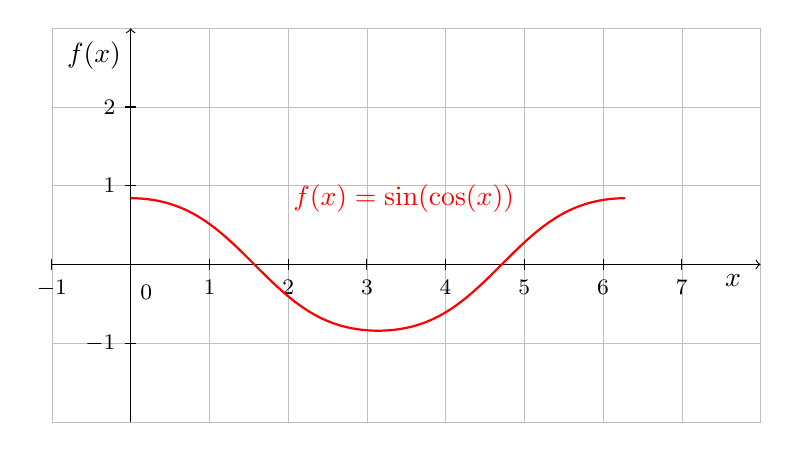
\begin{tikzpicture}[xscale=1, yscale=1]
	
	% Gitternetzlinien
	\draw[xstep=1cm, ystep=1cm, very thin, color=lightgray] (-1,3) grid (8,-2);
	% x-Achse
	\draw[->] (-1,0) -- (8,0) node[below,xshift=-1em] {$x$}; 
	%Zahlen auf x-Achse
	\foreach \x in {-1,...,-1}
	\draw[shift={(\x,0)},color=black] (0pt,2pt) -- (0pt,-2pt) node[below] {\footnotesize $\x$};
	\foreach \x in {1,...,7}
	\draw[shift={(\x,0)},color=black] (0pt,2pt) -- (0pt,-2pt) node[below] {\footnotesize $\x$};
	% y-Achse 
	\draw[->] (0,-2) -- (0,3) node[left,yshift=-1em] {$f(x)$};%node[above left]
	%Zahlen auf y-Achse
	\foreach \y in {-1,...,-1}
	\draw[shift={(0,\y)},color=black] (2pt,0pt) -- (-2pt,0pt) node[left] {\footnotesize $\y$};
	\foreach \y in {1,...,2}
	\draw[shift={(0,\y)},color=black] (2pt,0pt) -- (-2pt,0pt) node[left] {\footnotesize $\y$};
	%Ursprung
	\draw[color=black] (0pt,-10pt) node[right] {\footnotesize $0$};
	
	\draw[thick,color=red] plot[samples=200, domain=0:6.28] 
	(\x,{sin(cos(\x r)r}) node[ xshift=-8em]{$f(x)=\sin(\cos(x))$};
	
	
	\end{tikzpicture}
\end{center}
\subsection{Aufgabe 12 - Extrema bestimmen}
\href{https://youtu.be/cN-hCDhSnWw}{Video 14}\\
Gegeben sei:\\
\begin{align*}
f:\;\;]0,2\pi]\longmapsto\mathbb{R}\;\;\text{ mit}\;\;f(x)=\sin(\cos(x))
\end{align*}
Bestimme alle Extrema von $ f(x) $.\\
\\
$ \bullet $\;\;Extrema: \glqq innerer Punkte \grqq\\
\begin{quote}
	
	Bestimmung von $ f'(x) $:\\
	\begin{align*}
	f(x)&=\sin(\cos(x))\\
	f'(x)&=-\cos(\cos(x))\cdot \sin(x)
	\end{align*}
	Nullstellen von $ f'(x) $ bestimmen:\\
	$ f'(x) $ ist Null, wenn $ -\cos(\cos(x)) $ oder $ \sin(x) $ Null wird.\\
	Für $ -\cos(\cos(x)) $ gilt:
	\begin{align*}
	-\cos(\underbrace {\cos(x)}_{|\cos(x)|<1})
	\end{align*}
	Für $ \cos(x)=0 $ gilt:\\
	\begin{align*}
	&	\cos(x)=0\;\; \text{für }\;\;\frac{\pi}{2}+ n\cdot \pi\;\;\text{mit }\;\;n\in \mathbb{Z}\\
	&	\Rightarrow |\cos(x)|<\big|\frac{\pi}{2}+ n\cdot \pi\big|\;\;\text{mit }\;\;n\in \mathbb{Z}\\
	&\Rightarrow-\cos(\cos(x))\neq 0\;\;\text{für alle }\;\;x\in\mathbb{R}\\
	\end{align*}
	Für  $ \sin(x) =0$ gilt:\\
	\begin{align*}
	\sin(x)=0 \;\;\text{für }\;\;n\cdot\pi\;\;\text{mit }\;\;n\in \mathbb{Z}
	\end{align*}
	Wegen: $f:\;\;]0,2\pi]\longmapsto\mathbb{R}  $ existiert eine innere potenzielle Extremstelle: $ x_1=\pi $
\end{quote}
Bestimmung von $ f''(x) $:\\
\begin{align*}
f'(x)&=-\cos(\cos(x))\cdot \sin(x)\\
f''(x)&=-\sin(\cos(x))\cdot\sin(x)\cdot\sin(x)-\cos(x)\cdot\cos(\cos(x))\\
&=-\sin(\cos(x))\cdot\sin^2(x)-\cos(x)\cdot\cos(\cos(x))\\
\end{align*}
Bei der Extremstelle $ x_1=\pi $ gilt :\\
\begin{align*}
&f''(x)=-\sin(\cos(\pi))\cdot\underbrace {\sin^2(\pi)}_{=0}-\underbrace {\cos(\pi)}_{=-1}\cdot\underbrace {\cos(\cos(\pi))}_{=\cos(-1)>0}\\
&	f''(x)=0+1\cdot\cos(-1)>0\Rightarrow x_1=\pi\;\; \text{ist ein Minimum }
\end{align*}
Randpunkt und Grenzwertbetrachtung:\\
$ \bullet\;\;f(2\pi) =\sin(\cos(2\pi))=\sin(1)\Rightarrow \text{globales Maximum }$\\
$ \bullet\;\;f(\pi)\;\;=\sin(\cos(\pi)) =\sin(-1)=-\sin(1)\Rightarrow \text{ globales Minimum}$\\
$ \bullet\;\;\lim\limits_ {\substack{x\to 0\\x>0}} f(x)=\lim\limits_ {\substack{x\to 0\\x>0}}\sin(\cos(x))=\sin(1)$

\begin{center}
	
	
	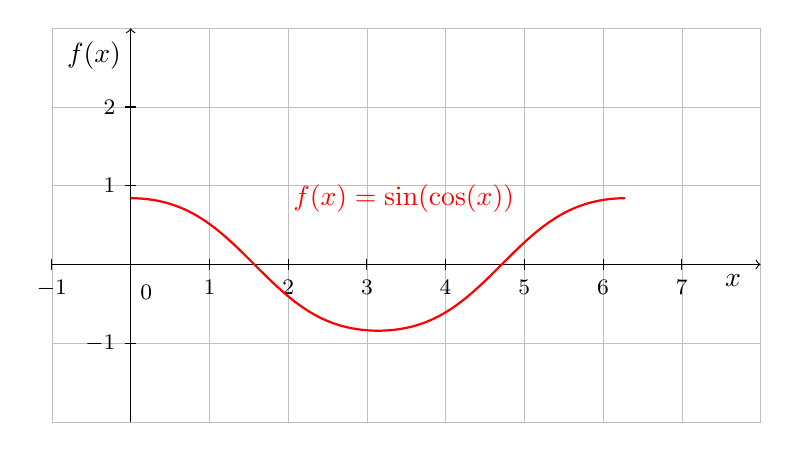
\begin{tikzpicture}[xscale=1, yscale=1]
	
	% Gitternetzlinien
	\draw[xstep=1cm, ystep=1cm, very thin, color=lightgray] (-1,3) grid (8,-2);
	% x-Achse
	\draw[->] (-1,0) -- (8,0) node[below,xshift=-1em] {$x$}; 
	%Zahlen auf x-Achse
	\foreach \x in {-1,...,-1}
	\draw[shift={(\x,0)},color=black] (0pt,2pt) -- (0pt,-2pt) node[below] {\footnotesize $\x$};
	\foreach \x in {1,...,7}
	\draw[shift={(\x,0)},color=black] (0pt,2pt) -- (0pt,-2pt) node[below] {\footnotesize $\x$};
	% y-Achse 
	\draw[->] (0,-2) -- (0,3) node[left,yshift=-1em] {$f(x)$};%node[above left]
	%Zahlen auf y-Achse
	\foreach \y in {-1,...,-1}
	\draw[shift={(0,\y)},color=black] (2pt,0pt) -- (-2pt,0pt) node[left] {\footnotesize $\y$};
	\foreach \y in {1,...,2}
	\draw[shift={(0,\y)},color=black] (2pt,0pt) -- (-2pt,0pt) node[left] {\footnotesize $\y$};
	%Ursprung
	\draw[color=black] (0pt,-10pt) node[right] {\footnotesize $0$};
	
	\draw[thick,color=red] plot[samples=200, domain=0:6.28] 
	(\x,{sin(cos(\x r)r}) node[ xshift=-8em]{$f(x)=\sin(\cos(x))$};
	
	
	\end{tikzpicture}
\end{center}
\subsection{Aufgabe 13 - Fourierpolynom}
\underline{Teil I}\\
\href{https://youtu.be/eVy5SC3mWBM}{Video 15 Teil 1}\\
Bestimme das $ n-k $ Fourierpolynom von:\\
\begin{align*}
f:\mathbb{R}\rightarrow\mathbb{R} \;\;\text{mit  }\;\; f(x)=\sin^2(x)\bigg(\cot^2(x)+\frac{1}{1-\cos^2(x)}\bigg)
\end{align*}
\\
Vereinfachung von $ f(x) $:\\
Es gilt:\\
\begin{align*}
\cot^2(x)&=\frac{\cos^2(x)}{\sin^2(x)}\\
1&=\cos^2(x)+\sin^2(x)\Leftrightarrow\sin^2(x)=1-\cos^2(x)\\
\cos(2x)&=\cos^2(x)-\sin^2(x)
\end{align*}
Eingesetzt ergibt sich dann:\\
\begin{align}
f(x)=\sin^2(x)\bigg(\frac{\cos^2(x)}{\sin^2(x)}+\frac{1}{\sin^2(x)}\bigg)=\cos^2(x)+1 \label{x1}
\end{align}
Ebenso gilt:\\
\begin{align}
\cos(2x)&=\cos^2(x)-\sin^2(x) \nonumber\\
\cos(2x)+1&=\cos^2(x)-\sin^2(x)+1\;\;|\scriptscriptstyle 1=\cos^2(x)+\sin^2(x)\nonumber\\
&=\cos^2(x)-\sin^2(x)+\sin^2(x)+\cos^2(x)\nonumber\\
&=2\cos^2(2x)\nonumber\\
\Leftrightarrow\nonumber\\
\cos^2(x)&=\frac{\cos(x)+1}{2}
\end{align}
(XV.2) in (XV.1) einsetzen:\\
\begin{align*}
f(x)&=\frac{\cos(2x)+1}{2}+1\\&=\frac{1}{2}\cos(2x)+\frac{1}{2}+1\\
f(x)&=\frac{3}{2}+\frac{1}{2}\cos(2x)
\end{align*}
Da $ f(x)=\frac{3}{2}+\frac{1}{2}\cos(2x) $ ein trigonometrisches Polynom ist, folgt:\\
\begin{align*}
\mathrm{Q}_n(x)=f(x)&=\frac{3}{2}+\frac{1}{2}\cos(2x)
\end{align*}
Bemerkung:\\
\begin{align*}
\mathrm{Q}_n(x)=\frac{a_0}{2}+\sum\limits_{k=1}^{n}a_k\cdot\cos(k\omega x)+b_k\cdot\sin(k\omega x)
\end{align*}
Bestimmung von $ \omega, a_k $ und $ b_k $ von $\mathrm{Q}_n(x)$ .\\
Für $ \omega $ gilt:\\
\begin{align*}
\omega =2\pi\cdot \mathrm{f}=\frac{2\pi}{\mathrm{T}}
\end{align*}
Der $ \cos(2x) $ ist $ \pi $-periodisch, daraus folgt:\\
\begin{align*}
&\Rightarrow \mathrm{T}=\pi\\
&\omega=\frac{2\pi}{\mathrm{T}}=\frac{2\pi}{\pi}=2
\end{align*}
Für $ a_0 $ gilt:\\
\begin{align*}
&\frac{a_0}{2}=\frac{3}{2}\\
&\Leftrightarrow\\
&a_0=3
\end{align*}
Für $ a_k $ gilt:\\ 
\begin{align*}
a_1=\frac{1}{2}\\
a_k=0\;\;\text{für }\;\; k>1
\end{align*}
Für $ b_k $ gilt:\\ 
\begin{align*}
b_k=0\;\;\text{für }\;\;k\geq 1
\end{align*}
Für $\mathrm{Q}_n(x)  $ gilt nun:\\
\begin{align*}
\mathrm{Q}_n(x)&=\frac{a_0}{2}+\sum\limits_{k=1}^{n}a_k\cdot\cos(k\omega x)+b_k\cdot\sin(k\omega x)\\
&=\frac{a_0}{2}+a_1\cos(k\omega x)+a_2\cos(k\omega x)\dots+b_1\sin(k\omega x)+b_2\cos(k\omega x)\dots\\
&=\frac{3}{2}+\frac{1}{2}\cos(1\cdot 2x)\\
\mathrm{Q}_n(x)=f(x)&=\frac{3}{2}+\frac{1}{2}\cos( 2x)\\
\end{align*}
\underline{Teil II}\\
\href{https://youtu.be/j2W_UAccyW8}{Video 16 Teil 2}\\
Bestimme  mit dem Fourierpolynom von:\\
\begin{align*}
f:\mathbb{R}\rightarrow\mathbb{R} \;\;\text{mit  }\;\; f(x)=\frac{3}{2}+\frac{1}{2}\cos(2x)
\end{align*}
das Integral:\\
\begin{align*}
\int\limits_{0}^{\pi} f(x)\cdot\sin(8x)\mathrm{d}x
\end{align*}
Es gilt für $ f(x) $:\\
\begin{align*}
b_k&=\frac{2}{\pi}\int\limits_{0}^{\pi} f(x)\cdot\sin(k\omega x)\mathrm{d}x\\
b_k&=0\;\;\text{ für}\;\;k\geq 0\\
\omega&=2\\
\Rightarrow&\\
b_k&=\frac{2}{\pi}\int\limits_{0}^{\pi} f(x)\cdot\sin(k\cdot2x)\mathrm{d}x\\
\end{align*}
Für $ b_k=4 $ gilt:\\
\begin{align*}
b_4&=\frac{2}{\pi}\int\limits_{0}^{\pi} f(x)\cdot\sin(4\cdot2x)\mathrm{d}x\;\;|\cdot\frac{\pi}{2}\\
&=\int\limits_{0}^{\pi} f(x)\cdot\sin(8x)\mathrm{d}x\
\end{align*}
Da $ b_4=0 $:\\
\begin{align*}
&b_4=\int\limits_{0}^{\pi} f(x)\cdot\sin(8x)\mathrm{d}x=0\\
&\Leftrightarrow\\
&\int\limits_{0}^{\pi} f(x)\cdot\sin(8x)\mathrm{d}x=0\\
\end{align*}
\subsection{Aufgabe 14 - Extrema bestimmen}
\href{https://youtu.be/9nOEDykwLso}{Video 17}\\
Bestimme alle Extrema von:\\
\begin{align*}
\mathrm{F}:\;\;]\genfrac{}{}{}{2}{1 }{2 },\infty[\;\;\longrightarrow \mathbb{R}\;\;\text{mit }\;\;\mathrm{F}(x)=\int\limits_{\frac{1}{2}}^{x} \ln(t)\mathrm{d}t
\end{align*}
$ \bullet $\;\;Extrema: \glqq innerer Punkte\grqq\\
\begin{quote}
	Bestimmung von $ \mathrm{F}'(x) $:
	\begin{align*}
	\mathrm{F}'(x)=\bigg(\int\limits_{\frac{1}{2}}^{x}\ln(t)\mathrm{d}t\bigg)'=\ln(x)
	\end{align*}
	Für die Nullstellen gilt :\\
	\begin{align*}
	\mathrm{F}'(x)=\ln(x)=0\;\;\text{für  }\;\;x_0=1
	\end{align*}
	Bestimmung von $ \mathrm{F}''(x) $:\\
	\begin{align*}
	\mathrm{F}''(x)=\bigg(\ln(x)\bigg)'=\frac{1}{x}
	\end{align*}
	Für  $ \mathrm{F}''(x)=\frac{1}{x}$ gilt:\\
	\begin{align*}
	&\frac{1}{x}\;\;\text{für }x\in [\genfrac{}{}{}{2}{1 }{2 },\infty]\;\;\text{gilt }\;\;\frac{1}{x}>0\\
	&\Rightarrow \mathrm{F}\;\;\text{ hat ein lokales Minimum bei:}\;\;x_0=1\\
	\end{align*}
\end{quote}
$ \bullet $\;\;Grenzwertbetrachtung:\\
\begin{quote}
	
	\begin{align*}
	\mathrm{F}(x)&=\int\limits_{\frac{1}{2}}^{x} \ln(t)\mathrm{d}t=\bigg[t(\ln(t)-1)\bigg]^x_{\frac{1}{2}}\;\;|\text{\tiny patielle Integration von $ \ln(t) $ }\\
	&=x(\ln(x)-1)-\frac{1}{2}(\ln(\genfrac{}{}{}{2}{1}{2})-1)
	\end{align*}
	$ \bullet \;\;\lim\limits_ {x\to\infty}\mathrm{F}(x)=\lim\limits_ {x\to\infty}x(\ln(x)-1)-\frac{1}{2}(\ln(\genfrac{}{}{}{2}{1 }{2 })-1)=\infty\Rightarrow\text{kein globales Maximum }$\\
	$ \bullet\;\;\lim\limits_ {\substack{x\to \frac{1}{2}\\x>\frac{1}{2}}}\mathrm{F}(x)= \lim\limits_ {\substack{x\to \frac{1}{2}\\x>\frac{1}{2}}}x(\ln(x)-1)-\frac{1}{2}(\ln(\genfrac{}{}{}{2}{1}{2 })-1)=0$
\end{quote}
Wenn der Funktionswert vom lokalen Minimum bei $ x_0=1 $  kleiner als Null ist, dann wird es wegen des  Grenzwertes bei $\lim\limits_ {\substack{x\to \frac{1}{2}\\x>\frac{1}{2}}}\mathrm{F}(x)= 0  $ ein globales Minimum.\\
Es gilt bei $ x_0=1 $:\\
\begin{align*}
\mathrm{F}(x)&=x(\ln(x)-1)-\frac{1}{2}(\ln(\genfrac{}{}{}{2}{1}{2})-1)\\
\mathrm{F}(1)&=1(\underbrace {\ln(1)}_{=0}-1)-\frac{1}{2}(\ln(\genfrac{}{}{}{2}{1}{2})-1)\\
&=-1-\frac{1}{2}\ln(\genfrac{}{}{}{2}{1 }{2 })+\frac{1}{2}=-\frac{1}{2}-\frac{1}{2}\ln(\genfrac{}{}{}{2}{1}{2 })=\frac{-1-\ln(\genfrac{}{}{}{2}{1 }{2 })}{2}=\frac{-1((\ln(1)-\ln(2)))}{2}\\
&=\frac{-1+\ln(2)}{2}
\end{align*}
Damit der Bruch kleiner Null wird, muß der $ \ln(2) <1$ sein:\\
Es gilt:\\
\begin{align*}
&\ln(2)<\ln(\mathrm{e})=1\\
&\Rightarrow\\
&\mathrm{F}(1)=\frac{-1+\ln(2)}{2}<0\\
&\Rightarrow\text{globales Minimum bei }\;\;x_0=1
\end{align*}
\subsection{Aufgabe 15 - Partialbruchzerlegung}
\href{https://youtu.be/H3AxdhKnQPc}{Video 18}\\
Bestimme alle Stammfunktionen von:\\
\begin{align*}
f(x)=\frac{x^4+4x^3+4}{x^4-1}
\end{align*}
Durch Erweiterung des Nenner mit $ +1-1 $ erreicht man,dass man im Zähler ein $ x^4-1 $ erhält und dies sich dann beim Zerlegenvon $ f(x) $ in einzelnen Summanten zu 1 kürzt.\\
\begin{align*}
f(x)=\frac{x^4-1+1+4x^3+4}{x^4-1}=\frac{x^4-1+4x^3+5}{x^4-1}
\end{align*}
Nun den Bruch in einzelne Summanten zerlegen:\\
\begin{align*}
f(x)=\frac{x^4-1+4x^3+5}{x^4-1}=\frac{x^4-1}{x^4-1}+\frac{4x^3}{x^4-1}+\frac{5}{x^4-1}=1+\frac{4x^3}{x^4-1}+\frac{5}{x^4-1}
\end{align*}
Nun die einzelnen Stammfunktion bilden:\\
$ \bullet $\;\;Stammfunktion von : $f_1(x) =1 $:\\
\begin{align*}
\mathrm{F}_1(x)=x+\mathrm{C}
\end{align*}
$ \bullet $\;\;Stammfunktion von : $f_2(x)=\frac{4x^3}{x^4-1}  $:\\
\begin{quote}
	Wenn im Zähler die Ableitung vom Nenner steht dann gilt:\\
	\begin{align*}
	\mathrm{F}_2(x)=\ln(x^4-1)+\mathrm{c}
	\end{align*}
\end{quote}
$ \bullet $\;\;Stammfunktion ohne Faktor 5 von: $f_3(x)=\frac{1}{x^4-1}   $\\

\begin{quote}
	Es gilt mit Partialbruchzerlegung für : $ f_3(x)=\frac{1}{x^4-1} $:\\
	\begin{align*}
	\frac{1}{x^4-1}=\frac{1}{(x^2-1)(x^2+1)}=\frac{1}{(x-1)(x+1)(x^2+1)}
	\end{align*}
	Es gilt:\\
	\begin{align*}
	\frac{1}{(x-1)(x+1)(x^2+1)}=\frac{\mathrm{A}}{x-1}+\frac{\mathrm{B}}{(x+1)}+\frac{\mathrm{C}x+\mathrm{D}}{(x^2+1)}
	\end{align*}
	Mit der \glqq Zuhaltemethode \grqq bekommt man:\\
	\begin{align*}
	\frac{1}{(1+1)(1^2+1)}=\frac{1}{4}=\mathrm{A}\\
	\frac{1}{(-1-1)(-1^2+1)}=-\frac{1}{4}=\mathrm{B}\\
	\end{align*}
	Durch einsetzen von A und B:\\
	\begin{align*}
	\frac{1}{(x-1)(x+1)(x^2+1)}&=\frac{\frac{1}{4}}{x-1}-\frac{\frac{1}{4}}{(x+1)}+\frac{\mathrm{C}x+\mathrm{D}}{(x^2+1)}\;\;|\cdot \scriptscriptstyle (x-1)(x+1)(x^2+1)\\
	1&=\frac{1}{4}(x+1)(x^2+1)-\frac{1}{4}(x-1)(x^2+1)+(\mathrm{C}x+\mathrm{D})(x-1)(x+1)\\
	&=\frac{1}{4}(x^3+x^2+x+1)-\frac{1}{4}(x^3-x^2+x-1)+(\mathrm{Cx}+\mathrm{D})(x^2-1)\\
		&=\frac{1}{4}(x^3+x^2+x+1)-\frac{1}{4}(x^3-x^2+x-1)+(\mathrm{C}x^3+\mathrm{D}x^2-\mathrm{C}-\mathrm{D})\\
	0\cdot x^3+	0\cdot x^2+	0\cdot x+1&=x^3\bigg(\frac{1}{4}-\frac{1}{4}+\mathrm{C}\bigg)+x^2\bigg(\frac{1}{4}+\frac{1}{4}+\mathrm{D}\bigg)+x\bigg(\frac{1}{4}-\frac{1}{4}-\mathrm{C}\bigg)+\frac{1}{4}+\frac{1}{4}-\mathrm{D}
	\end{align*}
	Mit Koeffizientenvergleich bekommt man:\\
	\begin{align*}
	0&=\frac{1}{4}-\frac{1}{4}+\mathrm{C}\Rightarrow\mathrm{C}=0\\
	1&=\frac{1}{4}+\frac{1}{4}-\mathrm{D}\Rightarrow\mathrm{D}=-\frac{1}{2}
	\end{align*}
	Für $ f_3(x) $ gilt nun:\\
	\begin{align*}
	f_3(x)&=\frac{1}{4}\bigg(\frac{1}{(x-1)}\bigg)-\frac{1}{4}\bigg(\frac{1}{(x+1)}\bigg)-\frac{1}{2}\bigg(\frac{1}{(x^2+1)}\bigg)\\
	\mathrm{F}_3(x)&=\frac{1}{4}\ln(x-1)-\frac{1}{4}\ln(x+1)-\frac{1}{2}\arctan(x^2+1)+\mathrm{c}
	\end{align*}
\end{quote}
Die Stammfunktionen von $ f(x) $ lauten nun:\\
\begin{align*}
\mathrm{F}(x)&=\mathrm{F_1}(x)+\mathrm{F_2}(x)+5(\mathrm{F_3}(x))\\
&=x+\ln(x^4-1)+5\bigg[\frac{1}{4}\ln(x-1)-\frac{1}{4}\ln(x+1)-\frac{1}{2}\arctan(x+1)\bigg]
\end{align*}




